\subsection{Addressing programs with Conditionals}
        We first consider programs with conditionals. The following two properties holds for any candidates of programs having conditional branching. 

        \begin{property}{Candidates of Programs with Conditionals}
            \label{CondB1}
            Let $B1$ be the sets of events based on a branch of a conditional in a program $P$. Let $C$ be any Candidate of $P$, Consider $b1$ to be representative of any event in $B1$ and an event $k$ outside the conditional branch. Then:
            \begin{align*}
                \exists C \in P \ \text{s.t.} b1 \notin C  
            \end{align*}
            There exists a candidate of the program such that events from the branch cannot be part of it\footnotemark. 
        \end{property}

        The above property is general for conditionals, being 1-branch or 2-branch. The latter however, has another property which we define below:

        \begin{property}{Candidates of Programs with Conditionals (2-branch)}
            \label{CondB2}
            Let $B1,B2$ be two sets of events based on each branch of a conditional in a program $P$. Let $C$ be any Candidate of $P$,  Consider $b1,b2$ to be representative of any event in $B1,B2$ respectively. Then:
            \begin{align*}
                \nexists C \in P \ \text{s.t.} \ b1 \in C \ \wedge \ b2 \in C \\ 
            \end{align*}
            There cannot exist any candidate of the program such that events from both sets can be part of it. 
        \end{property}

        The figure below summarizes the two forms of conditionals we can have in any program. 
        \begin{figure}[H]
            \centering 
            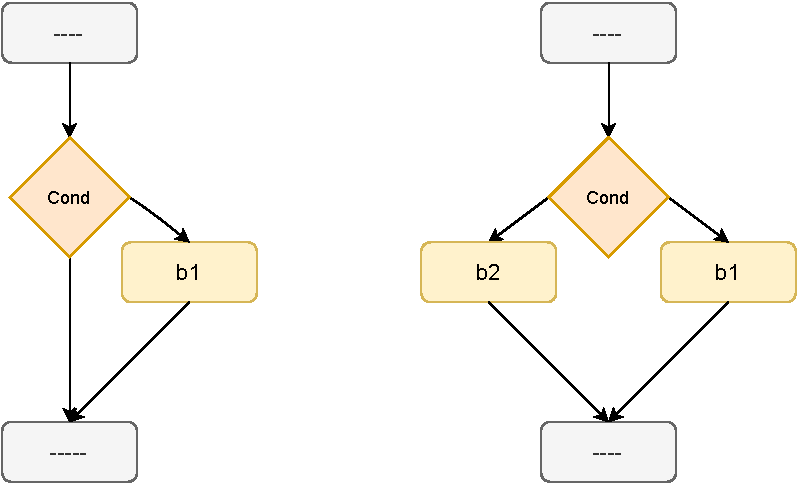
\includegraphics[scale=0.7]{5.InstructionReordering/5.ValidReorderingProgram/Conditionals2Form.pdf}
            \caption{Two forms of conditonals}
        \end{figure}

        \footnotetext{While the property for 1 branch may not always hold (it can be the case that the branch is always taken in any execution) we are defining it for any program.}

        We use the above two properties to state the following lemma 
        \begin{lemma}
            \label{CondBranchLemma}
            Reordering an event $e$ outside a conditional violates Property \ref{CondB1} and Property \ref{CondB2}
        \end{lemma}

        \begin{proof}
            
            Let $B1$ represent the set of events in a conditonal branch in program $P$ such that $e \in B1$. 
            
            Let us consider the first property. 
            By Property \ref{CondB1}, we have 
            \begin{align*}
                \exists C \in P \ \text{s.t.} \ \forall b \in B1, \ b \notin C
            \end{align*}

            On reordering event $e$ outside a conditional branch, we have 
            \begin{align*}
                \exists C \in P \ \text{s.t.} \ \forall b\!\neq\! e \in B1, \ b \notin C
            \end{align*}
            thus violating the Property \ref{CondB1} that must hold for the original program $P$.

            Now let us consider the second property. 
            Let $B2$ represent the set of events in the alternative branch to $B1$. 
            Then by Property \ref{CondB2}, we have 
            \begin{align*}
                \nexists C \in P \ \text{s.t} \ \forall b\!\in\!B2, \ e \in C \wedge b \in C
            \end{align*}

            On reordering event $e$ outside the conditional branch, we have 
            \begin{align*}
                \exists C \in P \text{s.t} \ \forall b\!\in\!B2, \ e \in C \wedge b \in C
            \end{align*}
            thus violating Property \ref{CondB2}, that must hold for the original program $P$.

        \end{proof}

        The above lemma's proof also lets us infer that on reordering an event outside a conditional, there are $new$ Candidates exist with a new event belonging to it. 
        We use this insight to state the following corollary for reordering under conditionals. 

        \begin{corollary}
            \label{ReordCond}
            Consider a program $P$ with conditional branches and its candidates $C_1, C_2, ... , C_n$ in which events $e$ and $d$ present in all of them with $\reln{e}{ao}{d}$. Consider the set of corresponding candidates $C'_1, C'_2, ... , C'_n$ after reordering $e$ and $d$ and its corresponding program $P'$. If the following two conditions hold:
            \begin{gather*}
                Reord(e,d) \ \wedge \ 
                ( \forall C_{i \in [1,n]}, \forall k \in C_i \ \text{s.t.} \ \reln{e}{ao}{k} \wedge \reln{k}{ao}{d}, \    
                Reord(e,k) \wedge Reord(k,d) ). \\
                \nexists C \in P \ s.t. \ 
                    (e \in C \ \wedge \ d \notin C) \ \vee \ 
                    (e \notin C \ \wedge \ d \in C). 
            \end{gather*}
            then the set of observable behaviors of $P'$ is a subset of that of $P$. 
        \end{corollary}

        \begin{proof}

            We prove the second condition first. 
            Assume the second condition does not hold. Then we would have
            \begin{align*}
                \exists C \in P \ s.t. \ 
                (e \in C \ \wedge \ d \notin C) \ \vee \ 
                (e \notin C \ \wedge \ d \in C).
            \end{align*}
            
            By Property \ref{CondB1}, $e$ or $d$ must belong to a conditional branch. 
            
            If $e$ and $d$ are in different branches of same conditonal, then by Prop \ref{CondB2} there wouldn't exist any candidate $C$ in $P$ where we could reorder $e$ and $d$. 
            If $e$ and $d$ are of the same conditonal branch, and neither one of them belong in any conditional branch nested within, then our above assumption does not hold. (simple sequential property of conditional branches)
            
            For the other cases, wihtout loss of generality, let us suppose the first condition holds, i.e. 
            \begin{align*}
                \exists C \in P \ s.t. \ 
                (e \in C \ \wedge \ d \notin C).
            \end{align*}
            The cases for the above can be summarized in the figure below:
            
            \begin{figure}[H]
                \label{CondCases}
                \centering 
                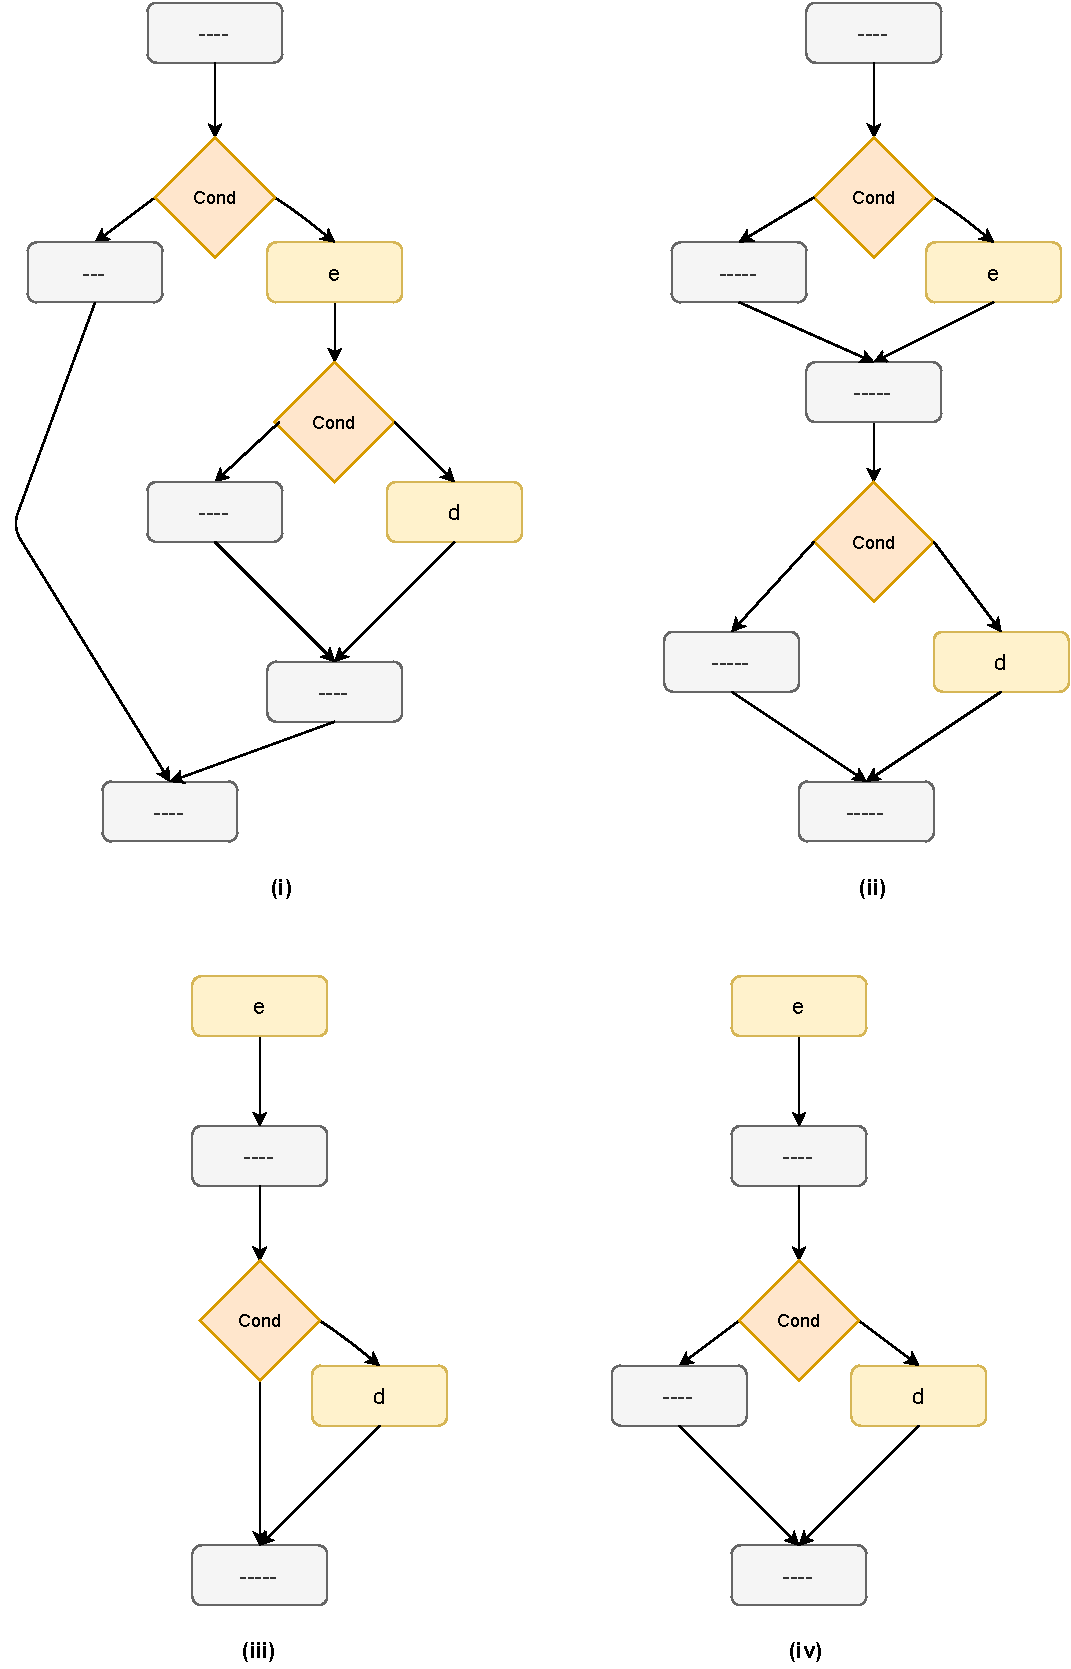
\includegraphics[scale=0.5]{5.InstructionReordering/5.ValidReorderingProgram/ConditionalCases.pdf}
                \caption{Four cases where $e$ or $d$ could be part of some conditional branch.}
            \end{figure}

            For cases (i) and (ii), by Lemma \ref{CondBranchLemma}, a new Candidate with event $e$ or $d$ exists without their respective conditional branches being taken.
            For cases (iii) and (iv), by Lemma \ref{CondBranchLemma}, a new Candidate with event $d$ exists without its respective conditional branch being taken.
            Irrespective of $e$ or $d$ being a read or a write, there could be a new $\stck{_{rf}}$ relation be formed with some event $k$ in the Candidate. By Def \ref{Obs}, we have a new observable behavior\footnotemark. 

            Hence, by contradiction, the second condition must hold.
            
            \footnotetext{Note that this argument is purely in terms of the execution graphs. The new event can possibly have a new reads-from relation established with some event in the graph itself. Since this new node did not exist in the graph before, and since every node in the graph is considered unique, we can infer that a new observable behavior is introduced. Analyzing which such execution graphs are equivalent, would imply drawing equivalence between two differnt reads-from relations. This could be done as a whole by addressing redundancy introduction optimization. This is not within the scope of the thesis.}

            Now that we have that the second condition must hold, we prove the first condition too must hold. Let $C_i$ and $C_i'$ be the candidates before and after reordering $e$ and $d$. From the first condition we have then for $C_i$
            \begin{align*}
                \forall \ k \ \textit{s.t.} \ 
                \reln{e}{ao}{k} \ \wedge \ \reln{k}{ao}{d} \ . \ 
                Reord(e,k) \ \wedge \ Reord(k,d).
            \end{align*}
            The above is Corollary \ref{CorollReord}, thus giving us that the observable behaviors of $C_i'$ is a subset of $C_i$. 
            By property of unions of sets, we can infer that the set of Observable Behaviors of $P'$ is a subset of that of $P$.

        \end{proof}
%------------------------------------------------------------------------------------------------------------------------------------------
    